\documentclass{ctexart}
\usepackage{amsmath}
\usepackage{amsfonts}
\usepackage{booktabs}
\usepackage{listings}
\usepackage{graphicx}
\begin{document}
\lstset{language=fortran}
\title{计算物理学第二次作业}
\author{谭淞宸 1700011706\thanks{tansongchen@pku.edu.cn}}
\date{2019.05}
\newcommand{\f}{\mathrm{d}}
\maketitle
\paragraph{作业摘要}
本文中,所有程序均使用 Fortran 90 编写,并在 Mac OS 10.14.4 的终端使用 gcc 8.3.0 中的 gfortran 模块编译。阅读提示:
\begin{enumerate}
    \item 第一题至第三题每题在 code 文件夹下设有一个文件夹(如 \verb|1/|);
    \item 第一题有一个模块文件 \verb|EigenProblem.f90| 和三个源代码文件 \verb|1_2.f90|, \verb|1_3.f90| 和 \verb|1_4.f90|;第二题有一个模块文件 \verb|Functions.f90| 和三个源代码文件 \verb|2_1.f90|, \verb|2_2.f90| 和 \verb|2_3.f90|;第三题有两个代码文件 \verb|3_2.f90| 和 \verb|3_3.f90|;每个代码文件对应一个无后缀的可执行文件。
    \item 所有代码文件均无输入文件,也不需要在执行过程中输入;
    \item 所有代码文件均对应输出文件 \verb|<可执行文件名>_output.txt|,提交时已经运行过并生成了相应的输出文件;
    \item 如需编译,请在 Mac OS 系统的命令行下转到相应目录并输入(例如第 1 题第 2 小题) \verb|gfortran 1_2.f90 -o 1_2|,这样会生成相应的无后缀可执行文件;继续输入 \verb|./1_2| 执行该文件;不推荐双击执行该文件,因为这可能导致工作目录(CWD)的错判进而无法在正确的位置读入和输出文件;
    \item 对于题目中涉及可变参数的情况,所有代码中均自动遍历所有参数,因此只需要运行 1 次。
\end{enumerate}
\newpage
\section{Mathieu 方程的本征值问题}
\subsection{实对称矩阵的实用 QR 算法}
\subsubsection{问题描述}
利用 Householder-Hessenberg 约化、Givens 旋转变换和原点位移构造一般实对称矩阵的 QR 算法。
\subsubsection{解答思路}
按讲义整理相关算法。在模块文件 \verb|Eigenproblem.f90| 中,包含如下四个子程序:
\begin{enumerate}
    \item \verb|subroutine EigenValues| 利用 QR 算法得到本征值;
    \item \verb|subroutine EigenVectors|利用反幂法改善本征值的精度并得到本征函数;
    \item \verb|subroutine LDL_Decomposition| 将一般实对称阵分解为 $\mathbf{LDL}^T$ 的形式,方便进行反幂法;
    \item \verb|subroutine Hamiltonian| 按题意构建 Hamilton 矩阵。
\end{enumerate}
\subsubsection{源代码}
见附录。
\subsection{本征值对参数的依赖性}
\subsubsection{问题描述}
求解下列 $2M+1$ 阶矩阵的本征值问题:
$$
\mathbf{H} \Psi=[\mathbf{T}+\mathbf{V}] \Psi=A \Psi
$$

其中动能矩阵

$$
T_{j k}=\left\{\begin{array}{ll}{(-1)^{j-k} \frac{\cos [\pi(j-k) /(2 M+1)]}{2 \sin ^{2}[\pi(j-k) /(2 M+1)]},} & {j \neq k} \\ {\frac{M(M+1)}{3},} & {j=k}\end{array}\right.
$$

势能矩阵

$$
V_{j k} \approx 2 q \cos \left(2 \phi_{j}\right) \delta_{j k}
$$

取 $M=50$,对参数 $q=[0,20]\cap\mathbb N$ 计算最小的 11 个本征值。
\subsubsection{解答思路}

依次调用 \verb|Hamiltonian|, \verb|EigenValues|, \verb|EigenVectors| 子程序即可。

\subsubsection{计算结果与讨论}
\begin{figure}[h]
\centering
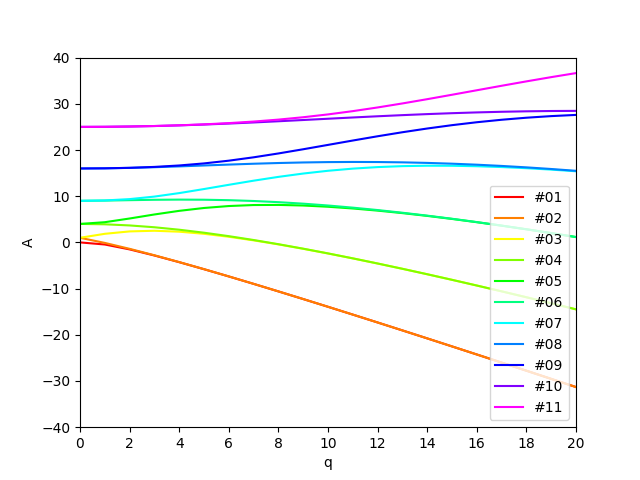
\includegraphics[scale=0.7]{101_qa.png}
\caption{$N=101$ 时 $A$ 与 $q$ 的关系}
\end{figure}

从图中可以看出,随着 $q$ 的增大,除基态外的二重简并(对应于谐振子本征值问题的正弦和余弦解)解除,并与相邻分支的本征值相互靠近,至 $q=20$ 时基本重新形成二重简并的结构(且基态也简并)。

\subsubsection{源代码}
\begin{lstlisting}
include 'EigenProblem.f90' 

program project1_2
    use EigenProblem
    implicit none
    integer i, j, k
    real*8, parameter :: q(0:20) = (/(i, i=0, 20)/)
    integer, parameter :: n = 101
    real*8 :: H(n,n), EV(n), top(11), Psi(n)

    open(10, file = '1_2_output.txt')
    call random_seed()
    do k = 0, 20
        ! 计算矩阵元
        call Hamiltonian(H, q(k), N)
        ! 计算本征值
        call EigenValues(H, EV)
        ! 选出最小的本征值
        do i = 1, 11
            top(i) = minval(EV)
            EV(minloc(EV)) = maxval(EV)
            ! 随机初始向量
            do j = 1, n
                call random_number(Psi(j))
            end do
            ! 利用反幂法优化本征值
            call EigenVectors(H, Psi, top(i))
        end do
        write(10, *) 'q=', q(k), top
        print *, 'q=', q(k), '计算完成'
    end do
end program
\end{lstlisting}
\subsection{解对格点数的收敛性}
\subsubsection{问题描述}
分别取 $M=5,40$,对比两种格点算出的最小的 5 个对应着偶宇称解的本征值,其余条件不变。
\subsubsection{解答思路}
我们只需在反幂法解出本征函数后判定其宇称即可。由于计算误差的存在,根据单点的函数值判断宇称有风险。但是我们注意到

$$
\phi_j+\phi_{N-j}=2\pi
$$

所以,我们可以令解 $\Psi[1:N-1:1]$ 和它的反向切片 $\Psi[N-1:1:-1]$ 作内积,如果结果为正,则应该为偶宇称,如果结果为负,则应该为奇宇称。

经初步试验,在一般情况下,奇宇称解和偶宇称解是交替的,且最低能级为偶宇称。这说明,我们最多只需要计算前 9 个本征值并挑出其中 5 个即可。

当 $q=0$ 或 $q>15$ 时,部分本征值接近简并,对应本征函数也简并,若采用反幂法计算收敛不到具有确定宇称的解。但是,这时由势场的性质和量子力学的基本规律(偶宇称势场简并态存在确定宇称的基本解组),我们知道可以取两个线性无关的本征函数,分别具有奇宇称和偶宇称,所以上述取法对于简并态也成立。

因此,在程序中我们不执行以上的判断偶宇称解的过程,而是简单地直接取按从小到大排列的本征值中的第 $2k+1(k\in \mathbb N)$ 个。
\subsubsection{计算结果与讨论}

\begin{figure}
\centering
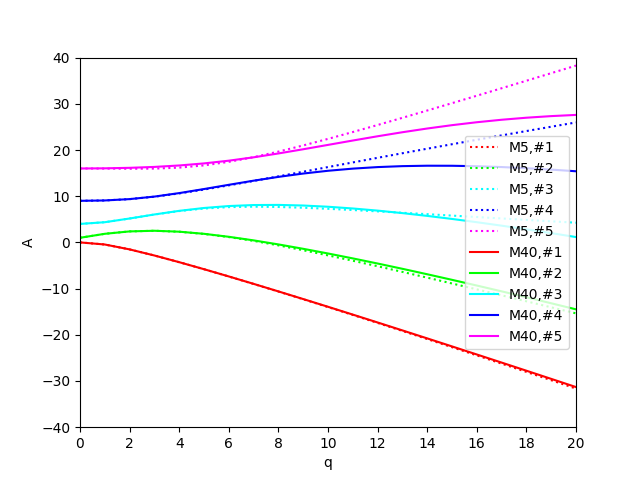
\includegraphics[scale=0.6]{5vs40.png}
\caption{$M=5,40$ 的本征值比较}
\end{figure}

从图片中可以看出,$q$ 较小时,两种格点得到的本征值差异不大,但 $q$ 较大时则产生了较大差异。从数学的角度看这是显然的($q$ 较大时势能项 $2q\cos2\phi$ 显著,由于它是余弦函数,振荡显著,必须用较多格点才能描述)。

~\\
~\\
\subsubsection{源代码}
\begin{lstlisting}
include 'EigenProblem.f90'

program project1_3
    use EigenProblem
    implicit none
    integer i, j, k, l, n
    real*8, parameter :: q(0:20) = (/(i, i=0, 20)/)
    integer, parameter :: n_list(2) = (/11, 81/)
    real*8, allocatable :: H(:,:), EV(:), Psi(:)
    real*8 :: top(9) = 0

    open(10, file = '1_3_output.txt')
    call random_seed()
    do l = 1, 2
        ! 确定格点数
        n = n_list(l)
        allocate(H(n,n),EV(n),Psi(n))
        do k = 0, 20
            call Hamiltonian(H, q(k), n)
            call EigenValues(H, EV)
            do i = 1, 9
                top(i) = minval(EV)
                EV(minloc(EV)) = maxval(EV)
                do j = 1, n
                    call random_number(Psi(j))
                end do
                call EigenVectors(H, Psi, top(i))
            end do
            ! 选出 5 个偶宇称解
            write(10, *) 'q=', q(k), top(1:9:2)
            print *, 'q=', q(k), '计算完成'
        end do
        deallocate(H,EV,Psi)
    end do
end program
\end{lstlisting}
\subsection{偶宇称本征函数}
\subsubsection{问题描述}
取 $M=50,q=10.0$,计算最小的 6 个对应着偶宇称解的本征值。
\subsubsection{解答思路}
计算过程与上一小问相同。
\subsubsection{计算结果与讨论}
~\\
~\\
\begin{table}[h]
\centering
\caption{最小的 6 个对应于偶宇称解的本征值}
\begin{tabular}{cc}
\toprule
序号 & 本征值\\
\midrule
\#01 & $-13.936552479241318$\\
\#02 & $-2.3821582359480540$\\
\#03 & $7.7173698497883390$\\
\#04 & $15.502784369741395$\\
\#05 & $21.104633708666722$\\
\#06 & $27.703768733948053$\\
\bottomrule
\end{tabular}
\end{table}


\begin{figure}[h]
\centering
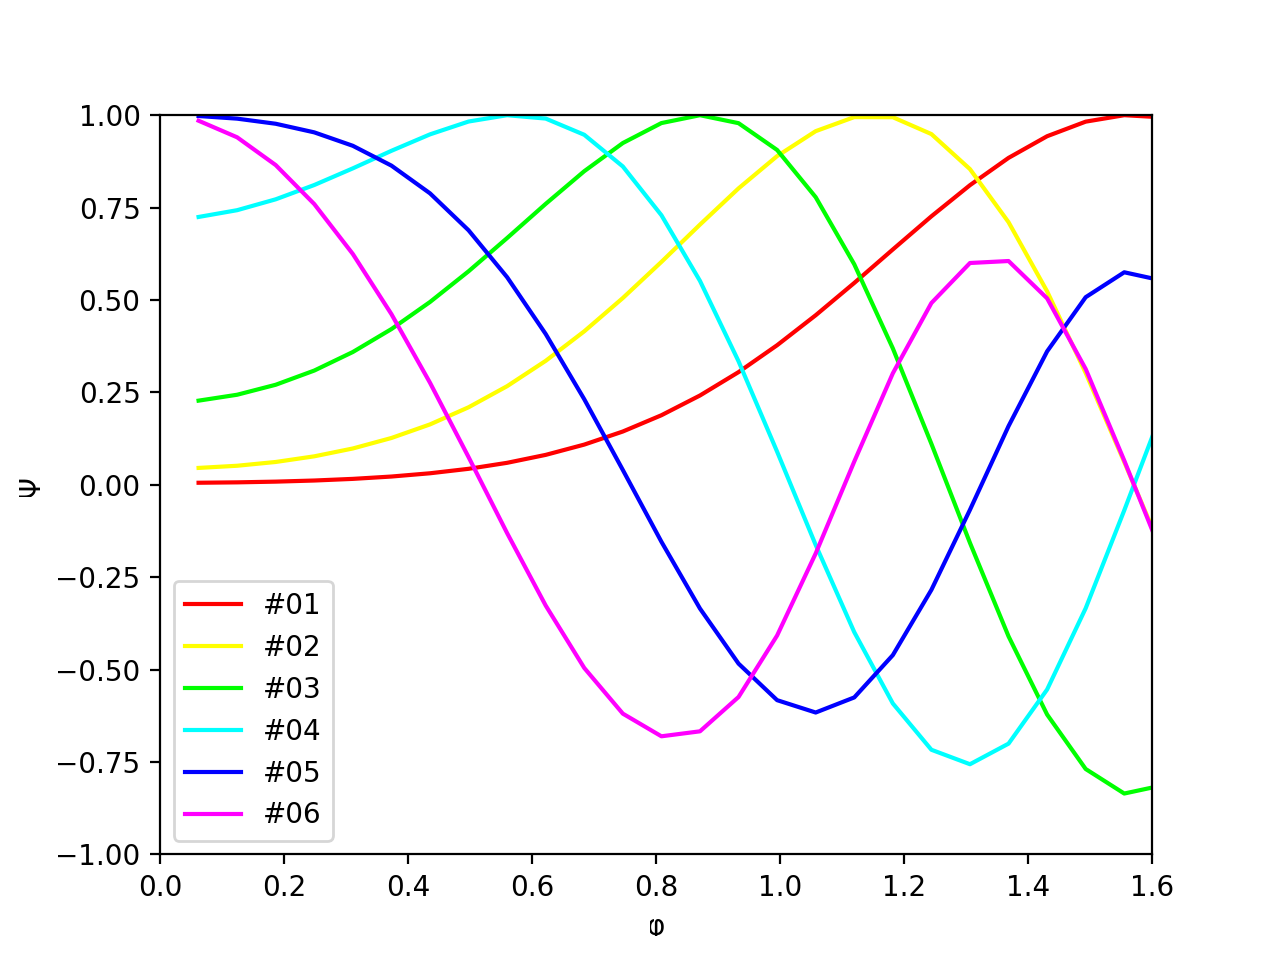
\includegraphics[scale=0.7]{even.png}
\caption{6 个偶宇称本征函数}
\end{figure}
\subsubsection{源代码}
\begin{lstlisting}
include 'EigenProblem.f90'

program project1_4
    use EigenProblem
    implicit none
    integer i, j, k, l
    real*8, parameter :: q = 10
    integer, parameter :: n = 101
    real*8 :: H(n,n), EV(n), Psi(n), top(11)

    open(10, file = '1_4_output.txt')
    call random_seed()
    call Hamiltonian(H, q, N)
    call EigenValues(H, EV)
    do i = 1, 11
        top(i) = minval(EV)
        EV(minloc(EV)) = maxval(EV)
        do j = 1, n
            call random_number(Psi(j))
        end do
        call EigenVectors(H, Psi, top(i))
        ! 输出本征值和本征函数
        if (mod(i,2) == 1) then
            write(10, *) top(i)
            write(10, *) Psi(1:N/4+1)
        end if
    end do
end program
\end{lstlisting}
\newpage
\section{激光场跃迁几率幅问题}
\subsection{鞍点方程求解}
\subsubsection{问题描述}
求如下鞍点方程的复数解,其中参数按作业中所给:

$$
S'(t)=\frac{1}{2}(\mathbf{p}+\mathbf{A}(\mathrm{t}))^{2}+\mathrm{I}_{\mathrm{p}}=0
$$

\subsubsection{解答思路}
由于是求复数解,我们采用 Müller 法(具体算法见附录)。考虑到 Müller 法每次只能得到一个解,我们先利用其他软件作图确定猜测解。猜测解精确到 100 个单位长度,实部分别为 $0,100,200,400,600,700$,虚部均为 $100$,然后在猜测解附近逐个求出。
\subsubsection{计算结果与讨论}
求出的 6 个解为(按实部从小到大):
\begin{itemize}
    \item $24.0598183 + 119.543541 i$
    \item $73.8798599 + 108.168762 i$
    \item $263.983368 + 36.8078499 i$
    \item $416.731934 + 27.8797989 i$
    \item $677.100891 + 64.2022858 i$
    \item $750.643738 + 84.5051117 i$
\end{itemize}

\subsubsection{源代码}
\begin{lstlisting}
include 'Functions.f90'

program project2_1
	use Functions
	implicit none
	! 进行初始猜测
	complex*8 :: guess(6) = &
	(/(0,100), (100,100), (200,100), &
	(400,100), (600,100), (700,100)/)
	complex*8 solution(6)

	open(10, file = '2_1_output.txt')
	call Muller(1.0D0, guess, solution)
	write(10, *) solution
end program
\end{lstlisting}
\subsection{鞍点法计算几率幅}
\subsubsection{问题描述}
利用如下鞍点近似公式计算几率幅。
$$
M_{\mathbf{p}}^{0}\left(t_{f}, t_{i}\right) _\mathrm{SP M}=-\frac{\left(2 I_{p}\right)^{\frac{5}{4}}}{\sqrt{2}} \sum_{\alpha} \frac{1}{S^{\prime \prime}\left(t_{s \alpha}\right)} e^{i S\left(t_{s \alpha}\right)}
$$
\subsubsection{解答思路}
求出 $S$ 和 $S''$ 的解析表达式。对于每个取定的 $p$ 值,代入鞍点方程(考虑到 $p$ 变化范围不大,猜测解可以不变),逐一求解即可。

\begin{align*}
S(t)&=\int_{0}^{t} d \tau\left[\frac{1}{2}(\mathbf{p}+\mathbf{A}(\tau))^{2}+I_{p}\right]\\
&=\frac1{6\omega}A_{0} p\left(3 \cos \left(\frac{t \omega}{2}\right)-3 \cos (t \omega)+\cos \left(\frac{3 t \omega}{2}\right)-1\right)\\
&+\frac{1}{960 \omega}A_{0}^{2}\left[90 t \omega-240 \sin \left(\frac{t \omega}{2}\right)+15 \sin (t \omega)+40 \sin \left(\frac{3 t \omega}{2}\right)\right.\\
&\left.-45 \sin (2 t \omega)+24 \sin \left(\frac{5 t \omega}{2}\right)-5 \sin (3 t \omega)\right]+\frac12p^{2} t+I_pt
\end{align*}

$$
S'(t)=\frac{1}{2}(\mathbf{p}+\mathbf{A}(\tau))^{2}+I_{p}
$$

$$
S''(t)=(\mathbf{p}+\mathbf{A}(\tau))\mathbf E(\tau)
$$

\subsubsection{计算结果与讨论(见 2.3.3)}
\subsubsection{源代码}
\begin{lstlisting}
include 'Functions.f90'

program project2_2
	use Functions
	implicit none
	integer i, j, k
	real*8 Prob, p_z
	real*8 :: p_range(200) = (/(i*1D-2, i=1, 200)/)
	complex*8 :: M, t
	complex*8 :: guess(6) = &
	(/(0,100), (100,100), (200,100), &
	(400,100), (600,100), (700,100)/)
	complex*8 solution(6)
	
	open(10, file = '2_2_output.txt')
	do i = 1, 200
		p_z = p_range(i)
		call Muller(p_z,guess,solution)
		M = 0
		! 进行对鞍点的求和
		do j = 1, 6
			t = solution(j)
			M = M + (2*I_p)**(5/4) / 2**0.5&
			*exp(Im*s(t,p_z)) / dds(t,p_z)
		end do
		! 计算几率
		Prob = abs(M)**2
		write(10, *) p_z**2/2, Prob
	end do
end program
\end{lstlisting}
\subsection{直接积分法计算几率幅}
\subsubsection{问题描述}
数值积分以下表达式:
$$
\begin{aligned} M_{\mathbf{p}}^{0}\left(t_{f}, t_{i}\right)_{\mathrm{D I}} &=\int_{t_{i}}^{t_{f}} d t\left\{\frac{\partial}{\partial \mathbf{q}}\left[\frac{2^{\frac{3}{2}}\left(2 I_{p}\right)^{\frac{5}{4}}}{\pi\left(\mathbf{q}^{2}+2 I_{p}\right)^{2}}\right]\right\} \cdot \mathbf{E}(t) e^{i S(t)} \\ &=2^{\frac{7}{2}}\left(2 I_{p}\right)^{\frac{5}{4}} \int_{t_{i}}^{t_{f}} d t \frac{\mathbf{q} \cdot \mathbf{E}(t)}{\pi\left(\mathbf{q}^{2}+2 I_{p}\right)^{3}} e^{i S(t)} \end{aligned}
$$
\subsubsection{解答思路}
采用变步长梯形积分公式,每次增加一倍格点,直至相邻两次积分数值之差小于某一给定误差限为止。
\subsubsection{计算结果与讨论}
\begin{figure}[h]
\centering
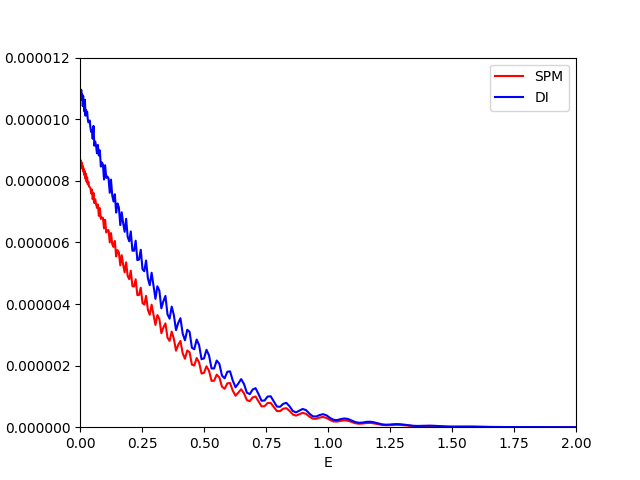
\includegraphics[scale=0.6]{spm_di.png}
\caption{鞍点法与直接积分法的比较}
\end{figure}

从图中可以看出,跃迁几率幅随末态电子动能增加而振荡下降,也即能量相差越大的态发生跃迁的概率越小(这是符合量子力学的一般规律的)。两种不同的方法所得曲线行为一致,仅仅相差一个约为 1.2 的倍数,且这一倍数在区间上基本保持不变,体现了方法之间的一致性。
\subsubsection{源代码}
\begin{lstlisting}
include 'Functions.f90'

program project2_3
	use Functions
	implicit none
	integer :: i, j, step
	real*8 Prob, p_z
	real*8 :: p_range(200) = (/(i*1D-2, i=1, 200)/)
	complex*8 :: tf = 4*pi/w, M, M_last
	complex*8, allocatable :: t(:)

	open(10, file = '2_3_output.txt')
	do i = 1, 200
		p_z = p_range(i)
		M = 1
		M_last = 0
		step = 1024
		! 变步长积分,每次增加一倍格点
		do while(abs(M_last-M)>1D-6)
			M_last = M
			step = step*2
			allocate(t(0:step))
			! 计算格点处函数值
			do j = 0, step
				t(j)=f(tf*j/step,p_z)
			end do
			! 梯形公式求积
			M = sum(t) / (step + 1) * tf
			deallocate(t)
		end do
		Prob = abs(M)**2
		write(10, *) p_z**2/2, Prob
	end do
end program
\end{lstlisting}
\newpage
\section{随机游走问题}
\subsection{一维游走的查点法}
\subsubsection{问题描述}
考虑一个醉汉从坐标原点出发。向左为负,向右为正,设步长为 1,每一步都与前一步无关。我们假定向左走一步的概率为 $q$,向右走一步的概率为 $p$。试表示出醉汉走了 3 步之后,离原点的距离 $x$ 的概率 $P$ 以及 $x$ 的期望值。
\subsubsection{解答思路}
距离满足二项分布 $B(p,3)$。显然:
\begin{itemize}
    \item 距离为 $-3$ 的概率为 $q^3$
    \item 距离为 $-1$ 的概率为 $3q^2p$
    \item 距离为 $1$ 的概率为 $3qp^2$
    \item 距离为 $3$ 的概率为 $p^3$
\end{itemize}
\subsection{二维格点游走的程序实现}
\subsubsection{问题描述}
醉汉从原点出发,且向上、下、左、右的概率是均等的,试编写程序描述这一过程,输出游走 50 步,每一步的坐标位置及距离原点的位移大小。
\subsubsection{解答思路}
利用内置函数生成 0 到 1 之间的随机数,根据它落入四个长度均等的子区间来判断向哪一个方向前进一步。
\subsubsection{计算结果与讨论}
从模拟结果(见 \verb|3_2_output.txt|)可以看出,随步数增加,位移的平均值增加,但具体关系还需进一步确定。
\subsubsection{源代码}
\begin{lstlisting}
program project3_2
	real*8 step(50), r ! 利用数组存储随机数
	integer :: x = 0, y = 0

	open(10, file = '3_2_output.txt')
	call random_seed()
	do i = 1, size(step)
		call random_number(step(i))
		! 判断随机数落入的子区间
		if (step(i) > 0.75) then
			x = x + 1
		else if (step(i) > 0.50) then
			x = x - 1
		else if (step(i) > 0.25) then
			y = y + 1
		else
			y = y - 1
		end if
		write(10, *) '第', i, '步游走后坐标 x = ', x, 'y = '&
		, y, '位移 r = ', sqrt(real(x)**2+real(y)**2)
	end do
end program
\end{lstlisting}
\subsection{二维任意游走的程序实现}
\subsubsection{问题描述}
考虑更一般的情況,假设醉汉从原点出发,可以向任一方向行走,步长依旧为 1, 每一步的位移方向与 $x$ 轴正方向的夹角为 $\theta$(假设这里的 $\theta$ 即为均匀分布的随机变量)。$n$ 步之后 $x$, $y$ 方向的位移,以及距离原点的距离分别为

$$
X_{n}=\sum_{k=1}^{n} \cos \theta_{k}, \quad Y_{n}=\sum_{k=1}^{n} \sin \theta_{k}, \quad R_{n}=\sqrt{X_{n}^{2}+Y_{n}^{2}}
$$

\subsubsection{解答思路}

仍利用内置函数生成随机数,并放大 $2\pi$ 倍成为角度,然后取相应的正弦和余弦即可。

拟合时,用最小二乘法,

$$
S=\sum_{i=1}^N\left(\langle R_i\rangle-a\sqrt i\right)^2
$$

$$
\frac{\partial S}{\partial a}=\sum_{i=1}^N-2\left(\langle R_i\rangle-a\sqrt i\right)\cdot\sqrt i=0
$$

$$
a=\frac{\sum_i\sqrt i\langle R_i\rangle}{\sum_i i}
$$

\subsubsection{计算结果与讨论}
通过运行 $10000$ 次取平均值的方法,计算得到 $a^* = 0.88669399410167160$,拟合情况如下:

\begin{figure}[h]
\centering
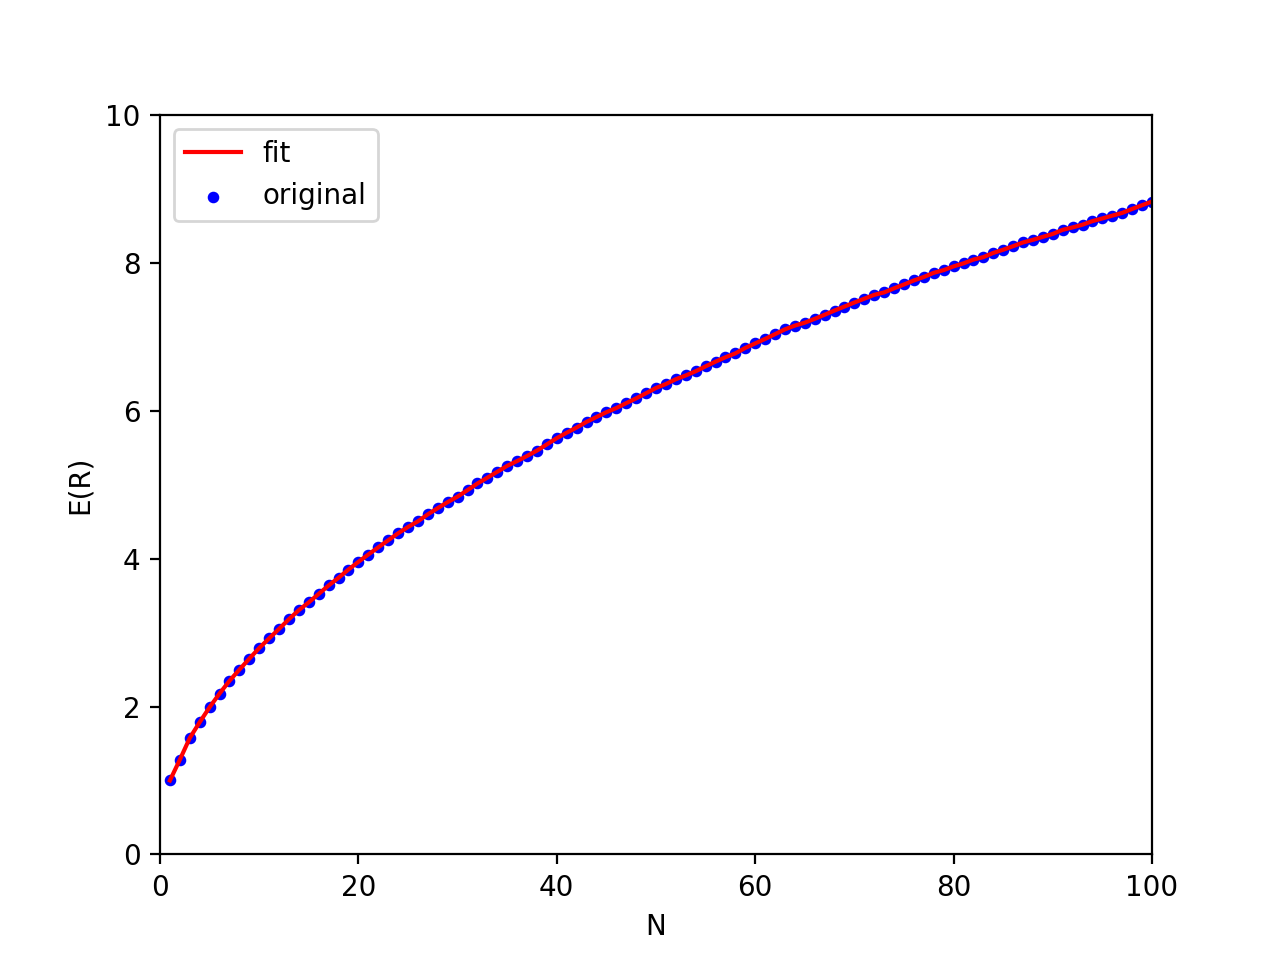
\includegraphics[scale = 0.5]{fit.png}
\caption{距离期望的拟合}
\end{figure}
\subsubsection{源代码}
\begin{lstlisting}
program project3_3
	real*8, parameter :: pi = 3.14159265358979323846D0
	integer, parameter :: steps = 100, tries = 10000
	real*8 :: step(steps), average(steps) = 0
	real*8 :: x = 0, y = 0, theta, r
	real*8 :: numbers(100) = (/(real(i), i = 1, 100)/)

	open(10, file = '3_3_output.txt')
	do j = 1, tries
		x = 0
		y = 0
		call random_seed()
		do i = 1, size(step)
			call random_number(step(i))
			! 将 [0,1] 之间的随机数转化为方位角
			theta = 2 * pi * step(i)
			x = x + cos(theta)
			y = y + sin(theta)
			r = sqrt(x**2+y**2)
			! 将距离录入平均值
			average(i) = average(i) + r
		end do
	end do
	! 计算平均值
	average = average / tries
	do i = 1, size(step)
		write(10, *) i, average(i)
	end do
	! 最小二乘法的公式实现
	write(10, *) '拟合参数为:', &
	sum(sqrt(numbers)*average)/sum(numbers)
end program
\end{lstlisting}
\subsection{坐标期望}
\subsubsection{问题描述}

试解析地证明 $X_n,Y_n$ 期望为 0,并计算它们的方差。
\subsubsection{解答思路}
在以下推导中,不带上下限的积分号表示对全范围积分,$\langle x^n\rangle_c$ 表示累积函数 cumulant,显然期望是 $\langle x\rangle_c=\langle x\rangle$,方差是 $\langle x^2\rangle_c$。

首先求出一步游走的概率分布函数($x$ 与 $y$ 相同):

\[
p(x)=\frac1{\pi\sqrt{1-x^2}}
\]

期望

\[
\mu=\langle x\rangle=\int x p(x)\f x=0
\]

方差

\[
\sigma^2=\langle x^2\rangle_c=\int (x-\langle x\rangle)^2 p(x)\f x=\frac12
\]

利用 Dirac Delta 函数可以将 $X_n$ 的概率分布函数表示成如下形式

\[
p(X_n)=\int \prod_{i=1}^n \f x_{i} p_i(x_i) \delta\left(X_n-\sum_{i=1}^{n} x_{i}\right)
\]

对它求期望,交换积分次序:

\begin{align*}
\langle X_n\rangle&=\int X_n p(X_n)\f X_n=\int X_n \f X_n
\int \prod_{i=1}^n \f x_{i} p_i(x_i) \delta\left(X_n-\sum_{i=1}^{n} x_{i}\right)
\\
&=\int \prod_{i=1}^n \f x_{i} p_i(x_i) \left(\sum_{i=1}^{n} x_{i}\right)=\sum_{i=1}^{n}\int x_{i}p_i(x_i)\f x_i=n\mu=0
\end{align*}

用同样的办法求方差:

\begin{align*}
\langle X_n\rangle_c&=\int \prod_{i=1}^n \f x_{i} p_i(x_i) \left(\sum_{i=1}^{n} x_{i}\right)^2
\\
&=\sum_{i=1}^{n}\int x_{i}^2p_i(x_i)\f x_i+\sum_{i\ne j}^{n}\int x_{i} x_{j} p_i(x_i) p_j(x_i)\f x_i\f x_j=n\sigma^2=\frac n2
\end{align*}

$x$ 与 $y$ 的概率密度函数仅差一个相位,因此 $Y_n$ 的各项数据与前述相同。

\subsection{独立性}
\subsubsection{问题描述}
试说明 $X_n,Y_n$ 是否相关、是否独立。
\subsubsection{解答思路}

由于每一步的 $\cos\theta, \sin\theta$ 是不独立的,因此 $X_n,Y_n$ 原则上是不独立的。例如,$n=1$ 时当 $X_n$ 确定后,$Y_n$ 就唯二地确定了($\pm\sqrt{1-X_n^2}$)。

但是,可以利用协方差证明它们的相关系数为 0:

$$
\operatorname{Cov}\left(X_{n}, Y_{n}\right)=\langle X_{n} Y_{n}\rangle-\langle X_{n}\rangle \langle Y_{n}\rangle=\langle X_{n} Y_{n}\rangle
$$

先求联合概率密度函数:

\[
p(X_n,Y_n)=\int \left[\prod_{i=1}^n \f x_{i}y_i p_i(x_i)p_i(y_i)\delta(x_i^2+y_i^2-1)\right] \delta\left(X_n-\sum_{i=1}^{n} x_{i}\right)\delta\left(Y_n-\sum_{i=1}^{n} y_{i}\right)
\]

进而求得期望:

\begin{align*}
\langle X_nY_n\rangle
&=\int X_nY_n p(X_n,Y_n)\f X_n\f Y_n
\\
&=\int\left[ \prod_{i=1}^n \f x_{i}\f y_i p_i(x_i)p_i(y_i)\delta(x_i^2+y_i^2-1)\right] \left(\sum_{i=1}^{n} x_{i}\right)\left(\sum_{i=1}^{n} y_{i}\right)
\end{align*}

上式中交叉项 $x_iy_j$ 直接积出显然为 0;对于非交叉项 $x_iy_i$,下列积分

\begin{align*}
&~~~~\int x_iy_i \f x_i \f y_i p_i(x_i) p_i(y_i)\delta(x_i^2+y_i^2-1)
\\
&=\int x_iy_i \f x_i \f y_i p_i(x_i) p_i(y_i)\left[\frac{\delta(x_i+\sqrt{1-y_i^2})}{2\sqrt{1-y_i^2}}+\frac{\delta(x_i-\sqrt{1-y_i^2})}{2\sqrt{1-y_i^2}}\right]
\\
&=\int \left[\sqrt{1-y_i^2}p_i\left(\sqrt{1-y_i^2}\right)+\left(-\sqrt{1-y_i^2}\right)p_i\left(-\sqrt{1-y_i^2}\right)\right] \frac{y_i}{2\sqrt{1-y_i^2}} \f y_i p_i(y_i)
\\
&=\int \left[p_i\left(\sqrt{1-y_i^2}\right)-p_i\left(-\sqrt{1-y_i^2}\right)\right] \frac{y_i}{2} \f y_i p_i(y_i)
\end{align*}


注意到 $p_i$ 是偶函数,因此上式被积函数为 0。

综上所述,我们证明了 $(X_n,Y_n)$ 的协方差为 0。
\subsection{正态分布近似}

\subsubsection{问题描述}
试解释为什么当 $n$ 的值足够大的时候,$(X_n,Y_n)$的联合概率密度可以表示成两个独立的正态分布的乘积的形式。
\subsubsection{解答思路}
我们定义新变量并给出它的累积函数(省略推导):

$$
\Xi_n=\frac{X_n-n\langle x\rangle}{n^{1 / 2}}
$$

$$
\langle \Xi_n\rangle=0
$$

$$
\left\langle \Xi_n^{k}\right\rangle_{c}=\left\langle x^{k}\right\rangle_{c} n^{1-n / 2}
$$

当 $n$ 非常大时,$n^{1-n / 2}\to0(n\ge3)$,所以我们在累积函数的生成函数中可以只考虑前两项(记 $\kappa_n$ 是相应于 $\Xi_n$ 的特性变量):

$$
\ln [p(\kappa_n)]=\sum_{k=0}^{\infty} \frac{(-i\kappa_n)^{k}}{k !}\left\langle \Xi^{k}\right\rangle_{c}=-\frac{\kappa^2\langle x^2\rangle_c}{2}=-\frac{\kappa^2\sigma^2}{2}
$$

从而 $p(\kappa_n)=\exp[-\frac{\kappa_n^2\sigma^2}{2}]$,对其进行逆 Fourier 变换得到

$$
p(\Xi_n)=\frac1{\sqrt{2\pi\sigma^2}}\exp[-\frac{\Xi_n^2}{2\sigma^2}]
$$

$$
p(X_n)=\frac1{\sqrt{2\pi n\sigma^2}}\exp[-\frac{X_n^2}{2n\sigma^2}]
$$

上面我们实际上利用中心极限定理证明了 $n$ 足够大时 $X_n$ 将符合正态分布。由于正态分布的形式仅与 $n,\sigma^2$ 有关,因此符合同一分布的 $Y_n$ 与它是独立的,联合概率密度可以写成它们的乘积:

$$
p(X_n,Y_n)=p(X_n)p(Y_n)=\frac{1}{2\pi n\sigma^2}\exp[-\frac{X_n^2+Y_n^2}{2n\sigma^2}]
$$

\subsection{$R^n$ 的概率密度函数和分布函数}

仍利用 Delta 函数:

$$
p(R_n)=\int \f X_n\f Y_n p(X_n,Y_n)\delta\left(X_n^2+Y_n^2-R_n^2\right)=\frac{R_n}{n\sigma^2}\exp[-\frac{R_n^2}{2n\sigma^2}]
$$

再进行积分即得到

$$
F(R_n)=\int_0^{R_n} p(R_n')dR_n'=1-\exp[-\frac{R_n^2}{2n\sigma^2}]
$$

\subsection{$R^n$ 的期望}

$$
\langle R_n\rangle=\int R_n p(R_n)\f R_n=-R\exp[-\frac{R_n^2}{2n\sigma^2}]\bigg|^\infty_0+\int\exp[-\frac{R_n^2}{2n\sigma^2}] \f R
$$

$$
\langle R_n\rangle=\sqrt{\frac{\pi n\sigma^2}{2}}
$$

由此看出,$\langle R_n\rangle$ 确实应该与 $\sqrt n$ 成线性关系,与我们的模拟结果一致。我们具体计算系数:

$$
a=\sqrt{\frac{\pi\sigma^2}2}=\sqrt{\frac\pi4}=0.8862269254527579
$$

可见我们拟合出的 $a^* = 0.88669399410167160$ 与真实的参数相比偏差约为 $0.04\%$。
\newpage
\appendix
\section{致谢}
感谢北京大学物理学院彭良友老师对于计算物理学知识详尽准确的介绍。

感谢北京大学物理学院刘士琦学姐、赵忠海学长针对作业进行的必要的提示以及回答我在编写程序时的疑问。
\newpage
\section{第一题模块源代码}
\begin{lstlisting}
module EigenProblem
contains
subroutine EigenValues(H, EV)
	implicit none
	integer j, k, n
	real*8 :: H(:,:), EV(:)
	real*8, allocatable :: a(:,:)
	real*8, allocatable :: x(:), x2(:,:), r(:,:)
	real*8, allocatable :: I(:,:), z(:,:), g(:,:)
	real*8 :: l = 0, c = 0, s = 0, d = 0

	n = size(H,1)
	allocate(a(n,n),r(n,n),I(n,n),z(n,n),&
		g(n,n),x(n),x2(n,1))
	! 复制一份矩阵,a 用来做运算,H 不变
	a = H

	! 单位矩阵
	I = 0
	forall (j=1:n) I(j,j) = 1
	! Householder 变换
	do j = 1, n-2
		x(:) = a(:,j)
		x(1:j) = 0
		if (x(j+1) > 0) then
			x(j+1) = x(j+1) + sqrt(dot_product(x,x))
		else
			x(j+1) = x(j+1) - sqrt(dot_product(x,x))
		end if
		x2 = spread(x,2,1)
		r = 2 * matmul(x2,transpose(x2)) / dot_product(x,x)
		a = a - matmul(r, a)
		a = a - matmul(a, r)
	end do
	k = n
	! Givens 变换
	do while (k > 1)
		! 判停标准
		if (abs(a(k,k-1)) < 1D-8) k = k - 1
		d = a(k,k)
		forall (j=1:k) a(j,j) = a(j,j) - d
		g = I
		do j = 1, k - 1
			c = a(j,j)/sqrt(a(j,j)**2+a(j+1,j)**2)
			s = a(j+1,j)/sqrt(a(j,j)**2+a(j+1,j)**2)
			z = I
			z(j,j) = c
			z(j+1,j+1) = c
			z(j,j+1) = s
			z(j+1,j) = -s
			a = matmul(z,a)
			g = matmul(z,g)
		end do
		a = matmul(a, transpose(g))
		forall (j=1:k) a(j,j) = a(j,j) + d
	end do
	! 保存到 EV 向量中
	forall (j=1:n) EV(j) = a(j,j)
	return
end subroutine

subroutine EigenVectors(H, v, p)
	implicit none
	integer i, j, k, n
	real*8 :: H(:,:), v(:)
	real*8, allocatable :: a(:,:), u(:)
	real*8 p, lambda

	n = size(H,1)
	allocate(u(n))
	a = H

	! 原点位移
	forall(i=1:n) a(i,i) = a(i,i) - p
	u = 0
	! LDL^T 分解
	call LDL_Decomposition(a)
	do while (dot_product(u-v,u-v) > 1D-8)
		! 解方程
		u = v
		do i = 1, n
			do k = 1, i-1
				v(i) = v(i) - a(i,k) * v(k)
			end do
		end do
		do i = n, 1, -1
			v(i) = v(i) / a(i,i)
			do k = i+1, n
				v(i) = v(i) - a(k,i) * v(k)
			end do
		end do
		! 近似特征值
		lambda = 1 / maxval(abs(v))
		! 规定在0到90度范围函数平均值大于0
		if (sum(v(1:n/4)) < 0) lambda = -lambda
		v = v * lambda
	end do
	p = p + lambda
end subroutine

subroutine LDL_Decomposition(a)
	implicit none
	integer i, j, k, n
	real*8 a(:,:)

	n = size(a,1)
	do i = 2, n
		! 非对角元,覆盖填入
		do j = 1, i-1
			do k = 1, j-1
				a(i,j) = a(i,j) - a(i,k) * a(j,k) * a(k,k)
			end do
			a(i,j) = a(i,j) / a(j,j)
		end do
		! 对角元,覆盖填入
		do k = 1, i-1
			a(i,i) = a(i,i) - a(i,k)**2 * a(k,k)
		end do
	end do
end subroutine

subroutine Hamiltonian(H, q, n)
	implicit none
	real*8 H(:,:)
	real*8, parameter :: pi = 3.14159265358979323846D0
	integer n, i, j
	real*8 q, t, v

	do i = 1, n
		do j = 1, n
			! 对角元
			if (i == j) then
				t = (n - 1) * (n + 1) / 12.0
				v = 2 * q * cos(4 * pi * j / n)
				H(i,j) = t + v
			! 非对角元
			else
				t = (-1)**(i - j) * cos(pi * (i - j) / n)&
				/ (1 - cos(2 * pi * (i - j) / n))
				H(i,j) = t
			end if
		end do
	end do
end subroutine
end module
\end{lstlisting}
\newpage
\section{第二题模块源代码}
\begin{lstlisting}
module functions
	! 题中所给常数
	real*8, parameter :: pi = 3.14159265358979323846D0
	real*8, parameter :: I_p = 0.5, &
	I_0 = 5D13, E_0 = sqrt(I_0/3.5094448314D16), &
	w = 4.55633525316D1/3.2D3, &
	A_0 = E_0 / w
	complex*8, parameter :: Im = (0,1)
contains

function A(t) ! 矢势
	complex*8 A, t
	A = A_0*sin(w*t)*sin(w*t/4)**2
	return
end function

function E(t) ! 电场
	complex*8 E, t
	E = -A_0*w*(cos(w*t)*sin(w*t/4)**2 +&
		sin(w*t)*sin(w*t/4)*cos(w*t/4)/2)
	return
end function

function s(t, p_z) ! S 函数
	complex*8 s, t
	real*8 p_z
	s = I_p*t + (90*A_0**2*t*w - 240*A_0**2*sin(w*t/2) +&
	    15*A_0**2*sin(w*t) + 40*A_0**2*sin(3*w*t/2) -&
	    45*A_0**2*sin(2*w*t) + 24*A_0**2*sin(5*w*t/2) -&
	    5*A_0**2*sin(3*w*t) + 480*A_0*p_z*cos(w*t/2) -&
	    480*A_0*p_z*cos(w*t) + 160*A_0*p_z*cos(3*w*t/2) +&
	    480*p_z**2*t*w - 160*A_0*p_z)/960/w
	return
end function

function ds(t, p_z) ! S 函数导数
	complex*8 ds, t
	real*8 p_z
	ds = (p_z+A(t))**2/2+I_p
	return
end function

function dds(t, p_z) ! S 函数二阶导数
	complex*8 dds, t
	real*8 p_z
	dds = -(p_z+A(t))*E(t)
	return
end function

function f(t, p_z) ! 直接积分法中的函数
	complex*8 f, t
	real*8 p_z
	f = 2**3.5*(2*I_p)**1.25*&
	exp(Im*s(t,p_z))*(p_z+A(t))*E(t)/&
	(pi*((p_z+A(t))**2+2*I_p)**3)
	return
end function

! 求根方法

subroutine Muller(p_z, guess, solution)
	implicit none
	integer :: i
	complex*8 x, y, z, sz
	complex*8 h, h0, h1, d, d0, d1
	complex*8 :: Delta, p, b
	! 初始猜测
	complex*8 :: guess(:), solution(:)
	real*8 :: p_z

	do i = 1, 6
		! 在初始猜测附近建立其它初始点
		y = guess(i)
		x = y - 10
		z = y + 10
		! 执行 Müller 法
		do while (.true.)
			h0 = x - z
			h1 = y - z
			sz = ds(z, p_z)
			d0 = (ds(x, p_z) - sz) / h0
			d1 = (ds(y, p_z) - sz) / h1
			d = (d0 - d1)/(h0 - h1)
			b = d0 - h0 * d
			Delta = sqrt(b**2 - 4*sz*d)
			if (abs(b-Delta) < abs(b+Delta)) then
				h = -2*sz/(b+Delta)
			else
				h = -2*sz/(b-Delta)
			end if
			p = z + h
			! 判停标准为解的变动幅度足够小
			! 这样能保证有 6 位有效数字
			if (abs(h) < 1D-4) then
				if (aimag(p) < 0) p = conjg(p)
				solution(i) = p
				exit
			else
				x = y
				y = z
				z = p
			end if
		end do
	end do
end subroutine
end module
\end{lstlisting}
\newpage
\end{document}